\documentclass[table,svgnames]{beamer}



\usepackage{graphicx}
\graphicspath{{0-images/}}
\usepackage{fancyvrb}
\usepackage{url}
\usepackage{xspace}
\PassOptionsToPackage{usenames,dvipsnames}{xcolor}
\usepackage{xcolor}
\usepackage{import}


\setlength{\leftmargini}{12pt}


\newcommand\link[1]{{\color{blue}#1}}



\RecustomVerbatimEnvironment{Verbatim}{Verbatim}{frame=single,fontsize=\scriptsize,commandchars=\\\{\}}


\usepackage{tikz}
\usepackage{tikz}
\usetikzlibrary{er,calc,positioning,shapes,shadows,arrows,shapes.callouts,backgrounds,fit}

\usetikzlibrary{arrows,shapes,shapes.callouts,positioning,backgrounds}
\usetikzlibrary{decorations.text}
\usetikzlibrary{shapes.arrows,shapes.symbols}
\usetikzlibrary{matrix}
\usetikzlibrary{fit}
\usetikzlibrary{calc}

\tikzset{
  invisible/.style={opacity=0},
  visible on/.style={alt=#1{}{invisible}},
  alt/.code args={<#1>#2#3}{%
    \alt<#1>{\pgfkeysalso{#2}}{\pgfkeysalso{#3}} 
  },
}

\tikzset{box/.style={rectangle,draw=#1!40,fill=#1!40,opacity=.9,rounded corners},box/.default=red}
\tikzset{boxFull/.style={rectangle,draw=#1!40,fill=#1!40,rounded corners},boxFull/.default=red}
\tikzset{lines/.style={draw=#1!80,ultra thick,rounded corners,opacity=.7},lines/.default=red}
\tikzset{balloon/.style={ellipse callout,fill=#1!50,opacity=.9},balloon/.default=red}
\tikzset{sqballoon/.style={rectangle callout,fill=#1!50,opacity=.9,rounded corners},sqballoon/.default=red}
\tikzset{sqballoonFull/.style={rectangle callout,fill=#1!50,rounded corners},sqballoonFull/.default=red}
\tikzset{cloud/.style={cloud callout, cloud puffs=150, aspect=2.5, cloud puff arc=120,shading=ball,text=white}}

\tikzstyle{na} = [baseline=-.5ex]
\tikzstyle{every picture}+=[remember picture]
\tikzstyle{every node}=[font=\large]
\tikzstyle{background grid}=[draw,black!50,step=1em]
\everymath{\displaystyle}

\usepackage{pgfplots}
\pgfplotsset{compat=1.7}


\pgfdeclarelayer{background}
\pgfdeclarelayer{foreground}
\pgfsetlayers{background,main,foreground}

\makeatletter
\pgfdeclareshape{document}{
  \inheritsavedanchors[from=rectangle] 
  \inheritanchorborder[from=rectangle]
  \inheritanchor[from=rectangle]{center}
  \inheritanchor[from=rectangle]{north}
  \inheritanchor[from=rectangle]{south}
  \inheritanchor[from=rectangle]{west}
  \inheritanchor[from=rectangle]{east}
  \inheritanchor[from=rectangle]{south east}
  %
  \backgroundpath{%
    %
    \southwest \pgf@xa=\pgf@x \pgf@ya=\pgf@y
    \northeast \pgf@xb=\pgf@x \pgf@yb=\pgf@y
    % 
    \pgf@xc=\pgf@xb \advance\pgf@xc by-5pt
    \pgf@yc=\pgf@yb \advance\pgf@yc by-5pt
    % 
    \pgfpathmoveto{\pgfpoint{\pgf@xa}{\pgf@ya}}
    \pgfpathlineto{\pgfpoint{\pgf@xa}{\pgf@yb}}
    \pgfpathlineto{\pgfpoint{\pgf@xc}{\pgf@yb}}
    \pgfpathlineto{\pgfpoint{\pgf@xb}{\pgf@yc}}
    \pgfpathlineto{\pgfpoint{\pgf@xb}{\pgf@ya}}
    \pgfpathclose
    % 
    \pgfpathmoveto{\pgfpoint{\pgf@xc}{\pgf@yb}}
    \pgfpathlineto{\pgfpoint{\pgf@xc}{\pgf@yc}}
    \pgfpathlineto{\pgfpoint{\pgf@xb}{\pgf@yc}}
    \pgfpathlineto{\pgfpoint{\pgf@xc}{\pgf@yc}}
  }
}
\makeatother

\tikzset{doc/.style={draw,document,text centered,text width=#1,inner sep=2ex, minimum width=1.5cm, minimum height=1cm },doc/.default=1cm }%



\newcommand{\documentSet}[3]{
  \begin{scope}
    \node[#1,fill=white,doc=.9cm] (#2) {#3};
    \begin{pgfonlayer}{background}
      \node[#1,doc=.9cm,yshift=-2pt, xshift=2pt] {#3};
      \node[#1,doc=.9cm,yshift=-4pt, xshift=4pt] {#3};
    \end{pgfonlayer}
\end{scope}
}

\newcommand{\documentSetL}[3]{
  \begin{scope}
    \node[#1,fill=white,doc=1.35cm] (#2) {#3};
    \begin{pgfonlayer}{background}
      \node[#1,doc=1.35cm,yshift=-2pt, xshift=2pt] {#3};
      \node[#1,doc=1.35cm,yshift=-4pt, xshift=4pt] {#3};
    \end{pgfonlayer}
\end{scope}
}





\PassOptionsToPackage{framemethod=TikZ}{mdframed}
\usepackage{mdframed}
\theoremstyle{definition}



\makeatletter
\pgfdeclareshape{document}{
  \inheritsavedanchors[from=rectangle] % 
  \inheritanchorborder[from=rectangle]
  \inheritanchor[from=rectangle]{center}
  \inheritanchor[from=rectangle]{north}
  \inheritanchor[from=rectangle]{south}
  \inheritanchor[from=rectangle]{west}
  \inheritanchor[from=rectangle]{east}
  \inheritanchor[from=rectangle]{south east}
  % 
  \backgroundpath{% 
    % 
    \southwest \pgf@xa=\pgf@x \pgf@ya=\pgf@y
    \northeast \pgf@xb=\pgf@x \pgf@yb=\pgf@y
    % 
    \pgf@xc=\pgf@xb \advance\pgf@xc by-5pt % 
    \pgf@yc=\pgf@yb \advance\pgf@yc by-5pt
    % 
    \pgfpathmoveto{\pgfpoint{\pgf@xa}{\pgf@ya}}
    \pgfpathlineto{\pgfpoint{\pgf@xa}{\pgf@yb}}
    \pgfpathlineto{\pgfpoint{\pgf@xc}{\pgf@yb}}
    \pgfpathlineto{\pgfpoint{\pgf@xb}{\pgf@yc}}
    \pgfpathlineto{\pgfpoint{\pgf@xb}{\pgf@ya}}
    \pgfpathclose
    % 
    \pgfpathmoveto{\pgfpoint{\pgf@xc}{\pgf@yb}}
    \pgfpathlineto{\pgfpoint{\pgf@xc}{\pgf@yc}}
    \pgfpathlineto{\pgfpoint{\pgf@xb}{\pgf@yc}}
    \pgfpathlineto{\pgfpoint{\pgf@xc}{\pgf@yc}}
  }
}
\makeatother

\tikzset{doc/.style={draw,document,text centered,text width=#1,inner sep=2ex, minimum width=1.5cm, minimum height=1cm },doc/.default=1cm }%



\usepackage{environ}
\makeatletter
\newsavebox{\measure@tikzpicture}
\NewEnviron{scaletikzpicturetowidth}[1]{%
  \def\tikz@width{#1}%
  \def\tikzscale{1}\begin{lrbox}{\measure@tikzpicture}%
  \BODY
  \end{lrbox}%
  \pgfmathparse{#1/\wd\measure@tikzpicture}%
  \edef\tikzscale{\pgfmathresult}%
  \BODY
}
\makeatother


%%% Local Variables:
%%% mode: latex
%%% TeX-master: "presentation"
%%% End:



\pgfdeclareimage[width=2.5cm]{XSPARQLogo}{0-images/XSPARQLLogo}



\pgfdeclareimage[width=1.5cm]{rdb}{0-images/Database.pdf}
\pgfdeclareimage[width=1cm]{rdb-table}{0-images/rdb.pdf}
\pgfdeclareimage[width=1.5cm]{xml}{0-images/XML.svg.pdf}
\pgfdeclareimage[width=1.5cm]{json}{0-images/json.pdf}
\pgfdeclareimage[width=1.5cm]{rdf}{0-images/rdf.pdf}
\pgfdeclareimage[width=1.5cm]{eat}{0-images/justeat.pdf}
\pgfdeclareimage[width=1.5cm]{excel}{0-images/excel.pdf}
\pgfdeclareimage[width=1.5cm]{dbpedia}{0-images/dbpedia.pdf}
\pgfdeclareimage[width=7cm]{lod}{0-images/lod.pdf}
\pgfdeclareimage[width=3cm]{map-pizza}{0-images/map-pizza.pdf}
\pgfdeclareimage[width=3cm]{deliveries}{0-images/spreadsheet.pdf}

\newcommand{\pgfscaleimage}[2]{\scalebox{#1}{\pgfuseimage{#2}}}


%%% Local Variables:
%%% mode: latex
%%% mode: flyspell
%%% mode: reftex
%%% TeX-master: "presentation"
%%% End:


\usepackage{listings}



\definecolor{orange}{RGB}{239,98,17}
\definecolor{green}{rgb}{0.10,0.60,0.08}


\mode<presentation>
{
  \usetheme[navigation=false]{DERI}
  \beamertemplateballitem
}



%%% Local Variables:
%%% mode: latex
%%% mode: flyspell
%%% mode: reftex
%%% TeX-master: "presentation"
%%% End:

\RecustomVerbatimEnvironment{Verbatim}{Verbatim}{frame=none,fontsize=\scriptsize}
\RecustomVerbatimCommand{\VerbatimInput}{VerbatimInput}{fontsize=\scriptsize}
\DefineVerbatimEnvironment{VerbatimChars}{Verbatim}{frame=none,fontsize=\scriptsize,commandchars=\\\{\}}


\newcommand{\fuzzyg}[2]{\mbox{$#1\colon#2$}}
\newcommand{\AU}{\ensuremath{\mathbf{U}}\xspace}
\newcommand{\AP}{\ensuremath{\mathbf{P}}\xspace}
\newcommand{\AB}{\ensuremath{\mathbf{B}}\xspace}
\newcommand{\AL}{\ensuremath{\mathbf{L}}\xspace}
\newcommand{\AV}{\ensuremath{\mathbf{V}}\xspace}
\newcommand{\AUBL}{\ensuremath{\mathbf{UBL}}\xspace}
\newcommand{\AUB}{\ensuremath{\mathbf{UB}}\xspace}
\newcommand{\AUL}{\ensuremath{\mathbf{UL}}\xspace}
\renewcommand{\AA}{\ensuremath{\mathbf{A}}\xspace}
\newcommand{\AULV}{\ensuremath{\mathbf{ULV}}\xspace}
\newcommand{\AUV}{\ensuremath{\mathbf{UV}}\xspace}
\newcommand{\triple}[1]{(#1)}
\newcommand{\term}[1]{\ensuremath{\mathrm{#1}}}
\newcommand{\eval}[1]{[\![ #1 ]\!]}
\newcommand{\ii}[1]{\mbox{$(#1)$}}
\renewcommand{\iff}{iff\xspace}
\newcommand{\rhodf}{\mbox{$\rho$df}\xspace}
\newcommand{\spp}{\ensuremath{\mathsf{sp}}}
\newcommand{\subclass}{\ensuremath{\mathsf{sc}}}
\newcommand{\type}{\ensuremath{\mathsf{type}}}
\newcommand{\dom}{\ensuremath{\mathsf{dom}}}
\newcommand{\range}{\ensuremath{\mathsf{range}}}
\newcommand{\typeR}{\ensuremath{\mathsf{type}}}


\newcommand{\I}{\ensuremath{\mathcal{I}}\xspace}      

\newcommand{\intL}[1]{{#1}^{\I_{L}} }
\newcommand{\intA}[1]{{#1}^{\I_{\A}} }
\renewcommand{\int}[1]{{#1}^{\I} }
\newcommand{\intP}[1]{{P[\![#1]\!]}}
\newcommand{\intC}[1]{{C[\![#1]\!]}}

\newcommand{\universe}{\ensuremath{\mathit{universe}}\xspace}
\newcommand{\tuple}[1]{\langle #1 \rangle }


\newcommand{\Vars}[1]{\ensuremath{\operatorname{vars}(#1)}}
\newcommand{\sem}[2]{\ensuremath{\left[\!\!\left[{#1}\right]\!\!\right]_{\mathit{#2}}}}
\newcommand{\semT}[3]{\ensuremath{\left[\!\!\left[{#1}\right]\!\!\right]_{\mathit{#2}}}^{\mathit{#3}}}
\newcommand{\xsparqlrewriter}{\ensuremath{\text{\textit{rewrite}}}}
\newcommand{\proofs}{\ensuremath{\vdash}}
\newcommand{\concat}{\ensuremath{\mathtt{fn{:}concat}}\xspace}
\newcommand{\rdfstyle}[1]{{\tt\textbf{#1}}}


\usepackage{bussproofs}
\def\stat{\ensuremath{\mathrm{statEnv}}}
\def\dyn{\ensuremath{\mathrm{dynEnv}}}
\newcommand{\statEnv}[1]{\stat \proofs #1}
\newcommand{\statEnvMultiline}[2]{\hspace{-5pt} \stat  \proofs \hspace{-7pt} \begin{array}{c} #1 \\ = \\ #2 \end{array}}
\newcommand{\dynEnv}[1]{\dyn \proofs #1}
\newcommand{\dynEnvMultiline}[2]{\hspace{-5pt} \dyn  \proofs \hspace{-7pt} \begin{array}{c} #1 \\ = \\ #2 \end{array}}

\newcommand{\ifThenElse}[3]{\ensuremath{\begin{array}{l}\mathtt{if}~(#1) \\ \indent \mathtt{then}~#2~\mathtt{else}~#3\end{array}}}
\newcommand{\fempty}[1]{\ensuremath{\mathit{fn{:}empty}(#1)}}
\newcommand{\envElem}[2]{\ensuremath{\mathit{#1}_{#2}}}
\newcommand{\var}[1]{\ensuremath{\$\mathit{#1}}}
\def\varname{\ensuremath{\var{VarName}}}



\def\XSPARQLFLWORExpr{\rdfstyle{Expr}\xspace}
\def\DECLARE{\rdfstyle{declare namespace}\xspace}
\def\FOR{\rdfstyle{for}\xspace}
\def\IN{\rdfstyle{in}\xspace}
\def\AT{\rdfstyle{at}\xspace}
\def\LET{\rdfstyle{let}\xspace}
\def\WHERE{\rdfstyle{where}\xspace}
\def\RETURN{\rdfstyle{return}\xspace}
\def\SATISFY{\rdfstyle{satisfy}\xspace}
\def\IF{\rdfstyle{if}\xspace}
\def\THEN{\rdfstyle{then}\xspace}
\def\ELSE{\rdfstyle{else}\xspace}
\def\WHERE{\rdfstyle{where}\xspace}
\def\SELECT{\rdfstyle{select}\xspace}
\def\ASK{\rdfstyle{ask}\xspace}
\def\FROM{\rdfstyle{from}\xspace}
\def\FROMNAMED{\rdfstyle{from named}\xspace}
\def\DESCRIBE{\rdfstyle{describe}\xspace}
\def\CONSTRUCT{\rdfstyle{construct}\xspace}
\def\DISTINCT{\rdfstyle{distinct}\xspace}
\def\ORDERBY{\rdfstyle{order by}\xspace}
\def\AND{\rdfstyle{and}\xspace}
\def\FILTER{\rdfstyle{filter}\xspace}
\def\OFFSET{\rdfstyle{offset}\xspace}
\def\LIMIT{\rdfstyle{limit}\xspace}
\def\UNION{\rdfstyle{union}\xspace}
\def\OPTIONAL{\rdfstyle{optional}\xspace}
\def\GRAPH{\rdfstyle{graph}\xspace}
\def\PREFIX{\rdfstyle{prefix}\xspace}
\def\BOUND{\rdfstyle{bound}\xspace} 
\def\isBlank{\rdfstyle{isBlank}\xspace} 
\def\isIRI{\rdfstyle{isIRI}\xspace}
\def\isLiteral{\rdfstyle{isLiteral}\xspace} 
\def\NULL{{\sf null}\xspace}


\newcommand{\set}[1]{\ensuremath{\mathbf{#1}}}
\newcommand{\uri}[1]{\ensuremath{\mathtt{#1}}}


\colorlet{sql}{green}
\colorlet{xquery}{green}
\colorlet{sparql}{green}
\colorlet{xsparql}{green}

\newcommand{\ecomp}[1]{\textrm{#1}}

\newcommand{\seq}[1]{\ensuremath{\left(#1\right)}}
\newcommand{\funcName}[1]{\ensuremath{\mathit{#1}}}
\newcommand{\funcCall}[2]{\ensuremath{\funcName{#1}\!\left(#2\right)}}
\newcommand{\e}[3]{\ensuremath{{\mathit{#1}}_{\mathit{#2}}^{\mathit{#3}}}}
\newcommand{\omg}[2]{\ensuremath{\e{\Omega}{#1}{#2}}}
\newcommand{\sm}[2]{\ensuremath{\e{\mu}{#1}{#2}}}
\newcommand{\grammarRule}[1]{{\textit{#1}}}
\def\DatasetClause{\grammarRule{Da\-ta\-set\-Clau\-se}\xspace}
\def\SparqlWhereClause{\grammarRule{Whe\-re\-Clause}\xspace}
\def\DatasetClause{\grammarRule{Da\-ta\-set\-Clau\-se}\xspace}
\def\OptDatasetClause{\grammarRule{Opt\-Dataset\-Clause}\xspace}
\def\SolutionModifier{\grammarRule{Solution\-Modifier}\xspace}
\newcommand{\envFunc}[2]{\ensuremath{\ecomp{#1}\!\left( #2 \right)}}
\newcommand{\envExtend}[2]{\ensuremath{\ecomp{ + }\envFunc{#1}{#2}}}


%%% Local Variables:
%%% mode: latex
%%% mode: flyspell
%%% mode: reftex
%%% TeX-master: "presentation"
%%% End:



\title{\Large{Integrating Heterogeneous Data by Extending Semantic Web Standards}}

\author{Nuno Lopes}

\date{26 November, 2012}


\begin{document}

\begin{frame}[plain]
  \titlepage
\end{frame}


\section{Overview}

\subsection*{}


\begin{frame}{Data Integration: Pizza Delivery Company} %on the Web

  \hspace*{-1em}
  \begin{tikzpicture}

    \begin{scope}[visible on=<+->]
      \node (rdb) at (5,-2) {\pgfuseimage{rdb}} ;
      \node at (rdb.north east) {\pgfuseimage{rdb-table}}; 
      \node[box=green,visible on=<.->] at (rdb.north west) {RDB};
      \node[inner sep=0,left=.1em of rdb.west] (rdb-name1) {Clients};
      \node[inner sep=0,below=.1em of rdb-name1.south] (rdb-name) {/ Orders};
      
      \begin{pgfonlayer}{background}
        \node[box=gray, fit=(rdb) (rdb-name)] (rdbms) {} ;
      \end{pgfonlayer}

      \begin{scope}[visible on=<+->]
        \node[boxFull=green,text width=3cm] at (rdb.south west) (rdb-order){
          {\small
            \begin{tabular}{c|c}
              person & address\\
              \hline
              Nuno & Galway \\
            \end{tabular}
          }
        };
      \end{scope}
      

    \end{scope}


    \begin{scope}[visible on=<+->]
      \node at (-4,-2) (excel) {\pgfuseimage{excel}};

      \node[inner sep=0] at (excel.south) (excel-name) {Deliveries};
      
      \begin{pgfonlayer}{background}
        \node[box=gray, visible on =<.->, fit=(excel) (excel-name)] {} ;
      \end{pgfonlayer}

      \node at (excel.north east) {\scalebox{.7}{\pgfuseimage{xml}}};
      \node[box=green,visible on=<.->] at (excel.north west) {XML};

      \node[visible on=<+->] at (excel.south east) {\pgfuseimage{deliveries}};
    \end{scope}

    
    \begin{scope}[visible on=<+->]
      \node (eat) at (-4,3){\pgfuseimage{eat}};
      \node[inner sep=0,below=.1em of eat.south] (eat-name1) {Clients};
      \node[inner sep=0,below=.1em of eat-name1.south] (eat-name) {/ Orders};

      \begin{pgfonlayer}{background}
        \node[box=gray, visible on =<.->, fit=(eat) (eat-name)] {} ;
      \end{pgfonlayer}

      \node[] at (eat.north east) {\scalebox{.7}{\pgfuseimage{xml}}};
      \node[boxFull=green] at (eat.north west) {XML};

      
      \node[boxFull=green,text width=4.2cm,anchor=north,visible on=<+->] at (eat.south east) (eat-order){
        \VerbatimInput[firstline=2,lastline=5]{queries/justeat.xml}
      };

    \end{scope}


    \node[visible on=<+>,anchor=north east] at (4,3) (dbpedia)  {\pgfuseimage{lod}};

    \begin{scope}[visible on=<+->]
      \node at (5,3) (dbpedia)  {\pgfuseimage{dbpedia}};

      \begin{pgfonlayer}{background}
        \node[box=gray, visible on =<.->, fit=(dbpedia)] {} ;
      \end{pgfonlayer}

      \node at (dbpedia.north east) {\scalebox{.7}{\pgfuseimage{rdf}}};
      \node[box=green,visible on=<.->] at (dbpedia.north west) {RDF};

    \end{scope}




    \begin{scope}[visible on=<+->]
      \node[boxFull=red,text width=7cm,visible on=<.>] at (1,1) (di)  {How many pizzas were delivered to Nuno's home during his PhD?};
      
      \path[-latex] (eat.south east) edge [color=xquery,line width=5pt] (di); 
      \path[-latex] (rdb.north west) edge [color=xquery,line width=5pt] (di); 
      \path[-latex] (excel.north east) edge [color=xquery,line width=5pt] (di); 
      \path[-latex,visible on=<.>] (dbpedia.south west) edge [color=xquery,line width=5pt] (di);
      
    \end{scope}
    
    \begin{scope}[visible on=<+->]
      \path[latex-latex] (dbpedia.south west) edge [color=xquery,line width=5pt] (di);
      \node at (di)  {\pgfuseimage{rdf}};
    \end{scope}

    
    \begin{scope}[visible on=<+->]
      \node[boxFull=red,anchor=north] at (eat-order.south){2012};
      \node[boxFull=red,anchor=south] at (rdb-order.north){From 2008 to 2012};
    \end{scope}


  \end{tikzpicture}

\end{frame}

\begin{frame}{Using Query Languages for Data Integration}

  \begin{tikzpicture}[scale=.9,transform shape]
    \matrix[ampersand replacement=\&, column sep = 4em,row sep=.5em ] {

      \node[visible on=<2->,text width=4.7cm] (sql) {
        \begin{block}{SQL}
          \VerbatimInput{queries/example.sql}
        \end{block}
      }; \&
      \node[right= of sql] (rdb) {\pgfscaleimage{.9}{rdb}}; 
      \\

      \node[visible on=<2->,text width=4.7cm] (sparql) {
        \begin{block}{SPARQL}
          \VerbatimInput[fontsize=\scriptsize]{queries/example.sparql}
        \end{block}
      };  \& 
      \node[right= of sparql] (rdf) {\pgfscaleimage{.9}{rdf}};
       \\

      \node[visible on=<2->,text width=4.7cm] (xquery) {
        \begin{block}{XQuery}
          \VerbatimInput{queries/example.xquery}
        \end{block}
      };  \& 
      \node[right= of xquery] (xml) {\pgfscaleimage{.9}{xml}};
       \\
    };
    \path[visible on=<2->,latex-] ([xshift=.5em]sql.east) edge [color=sql,line width=5pt] (rdb); 
    \path[visible on=<2->,latex-] ([xshift=.5em]sparql.east) edge [color=sparql,line width=5pt] (rdf); 
    \path[visible on=<2->,latex-] ([xshift=.5em]xquery.east) edge [color=xquery,line width=5pt] (xml); 

    \node[boxFull=green,visible on=<3->,anchor=south east] at (sql.south east) {relation};
    \node[boxFull=green,visible on=<3->,anchor=south east] at (sparql.south east) {solution sequence};
    \node[boxFull=green,visible on=<3->,anchor=south east] at (xquery.south east) {sequence of items};


    \draw[box=blue,visible on=<4->] let \p1 = (xquery.south west) in let \p2 = (sql.north west) in (\x1-5em,\y1) rectangle (\x1-3em,\y2) node[rotate=90,midway] (med) {Mediator / Data Warehouse};

    \foreach \point in {sql,sparql,xquery}
    { \path[visible on=<4->,-latex] ([xshift=1.1em]med.east |- \point) edge [color=orange,line width=5pt] (\point);  }

    \node[visible on=<5->] at (med.south west) {\pgfuseimage{rdf}};

    \node[boxFull=red,text width=6cm,visible on=<6->,left=6em of sparql,anchor=south,rotate=90] {How many pizzas were delivered to Nuno's home
      during his PhD?};


  \end{tikzpicture}
  
\end{frame}



\begin{frame}{How to represent context information in RDF?}

  \begin{itemize}
  \item RDF triples \\
    \begin{tabular}{ll}
      \begin{minipage}{0.5\paperwidth}
        \VerbatimInput[frame=single,fontsize=\scriptsize]{queries/address.ttl}
      \end{minipage}
      &
      \only<2->{
        \begin{minipage}{0.5\paperwidth}
          \alert{ Not enough!}
      \end{minipage}
    }
    \end{tabular}
    
    \item<3-> Domain vocabulary/ontology \\
      \begin{tabular}{ll}
        \begin{minipage}{0.5\paperwidth}
          \VerbatimInput[commandchars=\\\{\},fontsize=\scriptsize,frame=single]{queries/domain-vocab.ttl}
        \end{minipage}
        &
        \begin{minipage}{0.4\paperwidth}
          \only<6->{\alert{No defined \\semantics!}}
        \end{minipage}
      \end{tabular}

    \item<4-> Reification \\
      \begin{tabular}{ll}
        \begin{minipage}{0.5\paperwidth}
          \VerbatimInput[commandchars=\\\{\},fontsize=\scriptsize,frame=single]{queries/reification.ttl}
        \end{minipage}
        &
        \begin{minipage}{0.4\paperwidth}
          \only<6->{\alert{No defined \\semantics!}}
        \end{minipage}
      \end{tabular}

    \item<5-> Named Graphs

  \end{itemize}
\end{frame}

%%% Local Variables:
%%% mode: latex
%%% mode: flyspell
%%% mode: reftex
%%% TeX-master: "../presentation"
%%% End:








\begin{frame}{Hypothesis and Research Questions}

  \begin{block}{Hypothesis}%
    Efficient data integration over heterogenous data sources can be achieved by
    \begin{itemize}
    \item<2-> a combined query language that accesses heterogenous data in its original sources
    \item<3-> optimisations for efficient query evaluation for this language
    \item<4-> an RDF-based format with support for context information
    \end{itemize}
  \end{block}


  \begin{block}<5->{Research Questions}%
    \begin{itemize}
    \item<5-> How to design a query language that bridges the different formats?
    \item<6-> Can we reuse existing optimisations from other query languages?
    \item<7-> How to adapt RDF and SPARQL for context information?
    \end{itemize}
  \end{block}


\end{frame}





%%% Local Variables:
%%% mode: latex
%%% mode: flyspell
%%% mode: reftex
%%% TeX-master: "presentation"
%%% End:


{
  \setbeamertemplate{footline}{}
  \addtocounter{framenumber}{-1}
  \begin{frame}{Outline and Contributions} 
    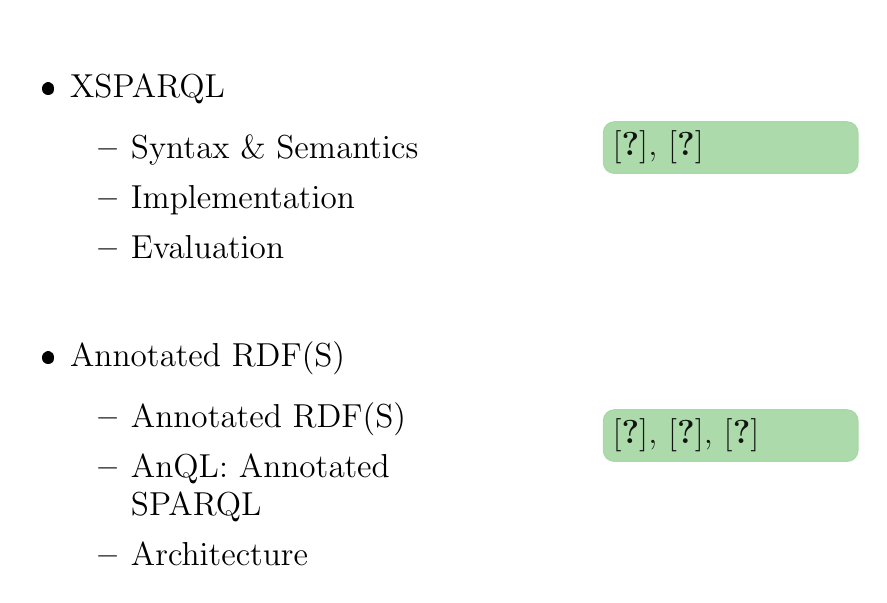
\begin{tikzpicture}
      \node[text width=.5\linewidth] (two) {
        \begin{itemize}
        \item XSPARQL
          \begin{itemize}
          \item Syntax \& Semantics
          \item Implementation
          \item Evaluation 
          \end{itemize}
        \end{itemize}
      };
      \node[box=green,right=of two,visible on=<2>,text width=3cm] {\cite{BischofDeckerKrennwallner:2012aa}, \cite{LopesBischofDecker2011aa}};
      \node[text width=.5\linewidth,below = 1em of two] (three){
        \begin{itemize}
        \item Annotated RDF(S)
          \begin{itemize}
          \item Annotated RDF(S)
          \item AnQL: Annotated SPARQL
          \item Architecture
          \end{itemize}
        \end{itemize}
      };
      \node[box=green,right=of three,visible on=<3>,text width=3cm] {\cite{StracciaLopesLukacsy:2010aa}, \cite{LopesPolleresStraccia:2010aa}, \cite{ZimmermannLopesPolleres:2012aa}};
    \end{tikzpicture}
  \end{frame}
}

\section{XSPARQL}
\subsection*{Overview}

\begin{frame}{XSPARQL}

    \begin{columns}
      \begin{column}{0.25\linewidth}
          \pgfuseimage{XSPARQLogo}
      \end{column}
      \begin{column}{0.65\linewidth}
        \begin{block}{}
          \begin{itemize}
          \item<+-> \alert<.>{Transformation language} between RDB, XML, and RDF
          \item<+-> \alert<.>{Syntactic} extension of XQuery
          \item<+-> \alert<.>{Semantics} based on XQuery's semantics
          \end{itemize}
        \end{block}
      \end{column}
    \end{columns}
    
    \vspace{10pt}

    \begin{block}<+->{Why based on XQuery? }
      \begin{itemize}
      \item<.-> Expressive language
      \item<.-> Use as scripting language
      \item<+-> Arbitrary Nesting of expressions
      \end{itemize}
    \end{block}

\end{frame}


\subsection{Syntax \& Semantics}
\begin{frame}{Same Language for each Format}

  \begin{center}
  \begin{tikzpicture}

    \node[visible on=<4>,text width=5.5cm] (xsparql) {
      \begin{block}{XSPARQL}
        \VerbatimInput{queries/example.sql.xsparql}
      \end{block}
    };

    \node[visible on=<5->,text width=5.5cm] (xsparql) {
      \begin{block}{XSPARQL}
        \VerbatimInput{queries/example.sparql.xsparql}
      \end{block}
    };

    \node[visible on=<2-3>,text width=5.5cm] (xsparql) {
      \begin{block}{\only<2>{XQuery}\only<3>{XSPARQL}}
        \VerbatimInput{queries/example.xquery}
      \end{block}
    };


    \node[box=green,visible on=<2>,text width=3cm,above =of xsparql.west] {
      {\small
        \begin{tabular}{l}
          \FOR \emph{var} \IN \emph{\XSPARQLFLWORExpr}\\
          \LET \emph{var} := \emph{\XSPARQLFLWORExpr}\\
          \WHERE \emph{\XSPARQLFLWORExpr}\\
          \ORDERBY \emph{\XSPARQLFLWORExpr}\\
          \RETURN \emph{\XSPARQLFLWORExpr}
        \end{tabular}}
    };

    \node[box=green,visible on=<4>,text width=3.5cm,above =of xsparql.west] {
      {\small
        \begin{tabular}{l}
          \FOR \emph{SelectSpec} \\
          \FROM \emph{RelationList} \\
          \WHERE \emph{WhereSpecList }\\ 
          \RETURN \emph{\XSPARQLFLWORExpr}
        \end{tabular}}
    };

    \node[box=green,visible on=<5>,text width=3.5cm,above =of xsparql.west] {
      {\small
        \begin{tabular}{l}
          \FOR \emph{varlist} \\
          \FROM~DatasetClause \\
          \WHERE \{\emph{ pattern } \}\\
          \RETURN \emph{\XSPARQLFLWORExpr}
        \end{tabular}}
    };


    \matrix[right =4em of xsparql,ampersand replacement=\&, column sep = 5em, row sep = 0, matrix of nodes] (matrix){
      
      \pgfuseimage{rdb} \\
      \pgfuseimage{rdf} \\
      \pgfuseimage{xml} \\ 
    };

    \path[visible on=<2->,latex-latex] ([xshift=.5em]xsparql.south east) edge [color=xsparql,line width=5pt] (matrix-3-1); 
    \path[visible on=<4->,-latex] ([xshift=.5em]xsparql.north east) edge [color=xsparql,line width=5pt] (matrix-1-1); 
    \path[visible on=<5->,-latex] ([xshift=.5em]xsparql.east) edge [color=xsparql,line width=5pt] (matrix-2-1); 

  \end{tikzpicture}
\end{center}
\end{frame}


\begin{frame}{Creating RDF with XSPARQL}
  
  \begin{tikzpicture}
    \node [text width=\linewidth] {
      \begin{block}<+->{Convert online orders into RDF}%
        \begin{tikzpicture}
        \node  [text width=\linewidth,]{
          \vspace{-1em}\VerbatimInput{queries/example_lifting.xsparql}
        };
        
        \begin{pgfonlayer}{background}
          \draw[box,visible on=<+>] (-0.51\linewidth,-0.6em) rectangle (0.45\linewidth,-1.5em);
        \end{pgfonlayer}

      \end{tikzpicture}

    \end{block}
    };

    \node[boxFull=green,text width=3cm,visible on=<.>] at (10.5em,-3em) {\CONSTRUCT{} clause generates RDF};
    \node[sqballoonFull,visible on=<+>,anchor=west, callout absolute pointer={(4.7em,-2.5em)},text width=4cm] at (2em,1em) {Arbitrary XSPARQL expressions in subject, predicate, and object};
  \end{tikzpicture}
  

\vspace{-5pt}

  \begin{block}<+->{Query result}
    \VerbatimInput{queries/example_lifting.xsparql.ttl}
  \end{block}

\end{frame}



\begin{frame}{Integration Query Example}
  
  \begin{block}{``Display pizza deliveries in Google Maps using KML''}
    \begin{tikzpicture}
      \node[text width=\linewidth]{\VerbatimInput{queries/example-integration.xsparql}};

      \begin{pgfonlayer}{background}
        \draw[box,visible on=<2>] (-0.51\linewidth,4.5em) rectangle (0.45\linewidth,3.5em);
        \draw[box,visible on=<3>] (-0.51\linewidth,3.6em) rectangle (0.45\linewidth,2em);
        \draw[box,visible on=<4>] (-0.51\linewidth,-1.9em) rectangle (0.45\linewidth,0em);
        \draw[box,visible on=<5>] (-0.51\linewidth,-1.8em) rectangle (0.45\linewidth,-4.9em);
      \end{pgfonlayer}
      \node[visible on=<2>] at (.35\linewidth,2.5em) {\scalebox{.7}{\pgfuseimage{xml}}};
      \node[visible on=<2>] at (.4\linewidth,3.5em) {\pgfuseimage{eat}};
      \node[visible on=<3>] at (.4\linewidth,2.2em) {\scalebox{.7}{\pgfuseimage{rdb}}};
      \node[visible on=<4>] at (.4\linewidth,0) {\scalebox{.7}{\pgfuseimage{rdf}}};
      \node[visible on=<5>] at (.35\linewidth,-2em) {\pgfuseimage{map-pizza}};

    
    \end{tikzpicture}
  \end{block}

  \begin{block}<6>{More involved XSPARQL queries: RDB2RDF}
    \begin{itemize}
    \item Direct Mapping: $\sim$130 LOC
    \item R2RML: $\sim$290 LOC
    \end{itemize}
  \end{block}

\end{frame}





\begin{frame}{Language Semantics}

  \begin{block}{}
    \begin{itemize}
    \item<1-> Extension of the XQuery Evaluation Semantics 
    \item<2-> \FOR{} add variables and values to the dynamic environment
    \item<3-> Reuse semantics of original languages for the new expressions
    \end{itemize}
  \end{block}


  \begin{tikzpicture}
    \node[text width=.95\linewidth]{
      \begin{block}{}
        \begin{tikzpicture}
          \node[text width=\linewidth]{\VerbatimInput{queries/example-integration.xsparql}};
          
          \begin{pgfonlayer}{background}
            \draw[box,visible on=<2>] (-0.51\linewidth,4.1em) rectangle (0.45\linewidth,3.2em);
          \end{pgfonlayer}

          \begin{pgfonlayer}{background}
            \draw[box,visible on=<3-5>] (-0.51\linewidth,3.2em) rectangle (0.45\linewidth,1.7em);
          \end{pgfonlayer}
          \node[boxFull=green,visible on=<4>,text width=3.5cm] at (0.35\linewidth,1em) {{\small  dynEnv.varValue  $\Rightarrow$ relation\\~ \\\begin{tabular}{l}person\\\hline "nuno"\end{tabular}}};
          \node[boxFull=green,visible on=<5>,text width=3cm] at (0.4\linewidth,3em) {{\small  eval(SQL SELECT) $\Join$ dynEnv.varValue}};

          \begin{pgfonlayer}{background}
            \draw[box,visible on=<6-7>] (-0.51\linewidth,0em) rectangle (0.45\linewidth,-1.6em);
          \end{pgfonlayer}
          \node[boxFull=green,visible on=<6>,text width=3.8cm] at (0.35\linewidth,-3.5em) {{\small dynEnv.varValue $\Rightarrow$ SPARQL sol. seq.\\\{\{~person~$\Rightarrow$~"nuno"~\}\}}};
          \node[boxFull=green,visible on=<7>,text width=3.8cm] at (0.35\linewidth,-3.5em) {{\small eval(SPARQL SELECT) solutions compatible dynEnv.varValue}};

        \end{tikzpicture}
      \end{block}
    };

    \node[visible on=<2>,anchor=east] at (-.45\linewidth,2.5em) {\scalebox{.4}{\pgfuseimage{xml}}};
    \node[visible on=<3-5>,anchor=east] at (-.44\linewidth,2em) {\scalebox{.4}{\pgfuseimage{rdb}}};
    \node[visible on=<6-7>,anchor=east] at (-.42\linewidth,0) {\scalebox{.4}{\pgfuseimage{rdf}}};

    \node[boxFull=beamer@lightblendedgreen,visible on=<8->,text width=\linewidth] {{\tiny
      \begin{prooftree}
        \def\ScoreOverhang{1pt}%
        \def\extraVskip{1pt}%
        \alwaysNoLine%
        % 
        \AxiomC{$\dyn.\ecomp{globalPosition} = \seq{ \envElem{Pos}{1}, \cdots, \envElem{Pos}{j} } $}
        % 
        \UnaryInfC{$\dynEnv{\funcCall{fs{:}dataset}{\DatasetClause} \Rightarrow \envElem{Dataset}{}}$}
        % 
        \UnaryInfC{$\begin{array}{r@{\hspace{-1pt}}l}%
            \dyn &~\proofs \funcCall{fs{:}sparql}{%
              \begin{array}{l}%
                \envElem{Dataset}{}, \SparqlWhereClause,\\
                \SolutionModifier
              \end{array}
            } \Rightarrow \sm{1}{}, \dots, \sm{m}{}
          \end{array}
          $}
        % 
        \UnaryInfC{$\begin{array}{r@{\hspace{-1pt}}l}%
            \dyn & \envExtend{globalPosition}{\seq{ \envElem{Pos}{1}, \cdots, \envElem{Pos}{j}, 1 }} ~\envExtend{activeDataset}{\grammarRule{Dataset}}\\
            &\envExtend{varValue}{%
              \begin{array}{l}%
                % \envElem{Variable}{pos} \Rightarrow 1;\\
                \envElem{Var}{1} \Rightarrow \funcCall{fs{:}value}{\sm{1}{},\envElem{Var}{1}};\\
                \dotsc;\\
                \envElem{Var}{n} \Rightarrow \funcCall{fs{:}value}{\sm{1}{},\envElem{Var}{n}}
              \end{array}%
            }~\proofs \grammarRule{ExprSingle} \Rightarrow
            \envElem{Value}{1}
          \end{array}$}
        % 
        \UnaryInfC{$\vdots$}
        % 
        \UnaryInfC{$\begin{array}{r@{\hspace{-1pt}}l}
            \dyn & \envExtend{globalPosition}{\seq{ \envElem{Pos}{1}, \cdots, \envElem{Pos}{j}, m }} ~\envExtend{activeDataset}{\grammarRule{Dataset}}\\
            &\envExtend{varValue}{\begin{array}{l}
                % \envElem{Variable}{pos} \Rightarrow n;\\
                \envElem{Var}{1} \Rightarrow \funcCall{fs{:}value}{\sm{m}{},\envElem{Var}{1}}; \\
                \dotsc; \\
                \envElem{Var}{n} \Rightarrow \funcCall{fs{:}value}{\sm{m}{},\envElem{Var}{n}} 
              \end{array}%
            }~\proofs \grammarRule{ExprSingle} \Rightarrow \envElem{Value}{m}
          \end{array}$}
        % 
        \singleLine
        % 
        \UnaryInfC{$\dynEnv{\begin{array}{l}
              \FOR~\envElem{\var{Var}}{1}\dotsb\envElem{\var{Var}}{n}~\DatasetClause\\
              \SparqlWhereClause~\SolutionModifier\\
              \RETURN~\grammarRule{ExprSingle}
            \end{array}} \Rightarrow \envElem{Value}{1}, \dots, \envElem{Value}{m}$}
      \end{prooftree}%
    }};

  \node[boxFull=red,visible on=<9->,text width=\linewidth] at (0,3.5em){{\tiny
      \vspace{-2em}%
      \begin{prooftree}%
        \def\ScoreOverhang{1pt}%
        \def\extraVskip{1pt}%
        \alwaysNoLine%
        % 
        \AxiomC{$\begin{array}{r@{\hspace{-1pt}}l}%
            \dyn &~\proofs \funcCall{fs{:}sparql}{%
              \begin{array}{l}%
                \envElem{Dataset}{}, \SparqlWhereClause,\\
                \SolutionModifier
              \end{array}
            } \Rightarrow \sm{1}{}, \dots, \sm{m}{}
          \end{array}
          $}
      \end{prooftree}%
    }};

  \end{tikzpicture}
\end{frame}



%%% Local Variables:
%%% mode: latex
%%% mode: flyspell
%%% mode: reftex
%%% TeX-master: "../presentation"
%%% End:



\begin{frame}{Language Implementation}

  \begin{block}{}
    \begin{itemize}
    \item<1-> Reuse components (SPARQL engine, Relational Database)
    \item<2-> Implemented XSPARQL by rewriting to XQuery
    \item<3-> Semantics implemented by substitution of bound variables
    \end{itemize}
  \end{block}

  \begin{block}<4->{Bound Variable Substitution}
    \begin{itemize}
    \item<4-> \alert{Bound} variables are replaced by their \alert{value} at runtime
    \item<5-> Implemented in the generated XQuery
    \item<6-> Pushing the variable bindings into the respective query engine
    \end{itemize}
  \end{block}

  \begin{block}<4->{}
    \begin{tikzpicture}
      \node[text width=\linewidth]{\vspace*{-1em}\VerbatimInput[lastline=3]{queries/example-integration.xsparql}};

      \begin{pgfonlayer}{background}
        \draw[box,visible on=<4>] (-13em,.5em) rectangle (-9.5em,1.5em);
        \draw[box,visible on=<4>] (-4em,0em) rectangle (-8em,-1em);

        \draw[box,visible on=<5-6>] (-0.51\linewidth,-1em) rectangle (0.45\linewidth,.5em);

      \end{pgfonlayer}

      \node[boxFull=green,visible on=<5-6>,text width=4.7cm,anchor=west] at (1em,-1em) {\vspace*{-1em}\VerbatimInput[firstline=2,lastline=4]{queries/variable-replacement.xq}};

    
    \end{tikzpicture}
  \end{block}


\end{frame}


\subsection{Implementation}


\begin{frame}{Implementation}

  \begin{center}
    
  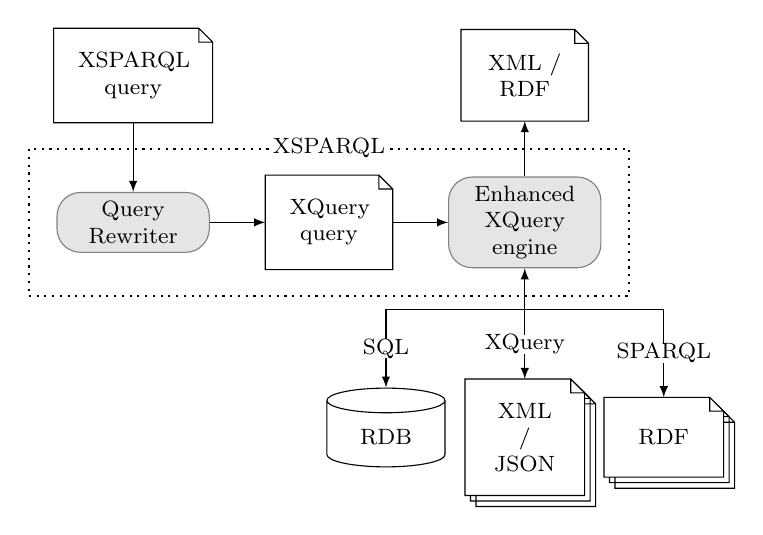
\begin{tikzpicture}[
    terminal/.style={ rectangle,minimum size=6mm,rounded corners=3mm,text centered,draw=black!50,fill=gray!20},%
    rdb/.style={cylinder, shape border rotate=90, draw,minimum width=1.5cm,minimum height=1cm, shape aspect=.35}%
    ]
    \tikzstyle{every node}=[font=\footnotesize]


    % XSPARQL engine
    \begin{scope}[node distance = 20pt]
      \node[terminal,text width=1.7cm] (rewriter) {Query Rewriter}; %
      \node[right=of rewriter,doc=1cm] (rewritenXQ) {XQuery query};%
      \node[right=of rewritenXQ, terminal,text width=1.7cm] (EXQuery) {Enhanced XQuery engine}; %
    \end{scope}


    % XSPARQL query
    \node[above=2.5em of rewriter, doc=1.4cm] (XS-Q) {XSPARQL query};%

    \coordinate[below=1.5em of EXQuery.south] (input-separator);
    % input sources
    \begin{scope}[node distance = 7pt]
      \documentSet{below=2.5em of input-separator}{xml}{XML / JSON};
      \documentSet{right=of xml}{rdf}{RDF};
      \node[left=of xml, rdb]  (rdb)  {RDB};%
    \end{scope}
  
    \draw[-latex] (input-separator) -- (EXQuery.south);%
    \draw[-latex] (input-separator) -- (xml.north) node [midway,inner sep=0,fill=white] {XQuery};%
    \draw[-latex] (input-separator) -| (rdb.north) node [near end,inner sep=0,fill=white] {SQL};%
    \draw[-latex] (input-separator) -| (rdf.north) node [near end, inner sep=0,fill=white] {SPARQL};%

    % outputs
    \begin{scope}[node distance = 2pt]
      \node[above=2em of EXQuery, doc=1cm] (output) {XML~/ RDF};%
    \end{scope}
  
    % inner diagram arrows
    \draw[-latex] (rewriter.east) -- (rewritenXQ.west);%
    \draw[-latex] (rewritenXQ.east) -- (EXQuery.west);%
    
    % outer box
    \node[draw=black,dotted,thick,inner sep=10pt,rectangle,fit=(rewriter) (EXQuery)] (XSPARQL) {} ;%
    \node[inner sep=0,fill=white] at (XSPARQL.north) {XSPARQL};

    % outer diagram arrows
    \draw[-latex] (XS-Q.south) -- (rewriter.north);%

    % output lines
    \draw[-latex] (EXQuery.north) -- (output.south) ;%

  \end{tikzpicture}

%%% Local Variables:
%%% mode: latex
%%% mode: flyspell
%%% mode: reftex
%%% TeX-master: "../thesis"
%%% End:


  \end{center}
  
\end{frame}



\subsection{Evaluation}

\begin{frame}{XSPARQL Evaluation}

  \vspace{-5pt}

  \begin{center}{}
    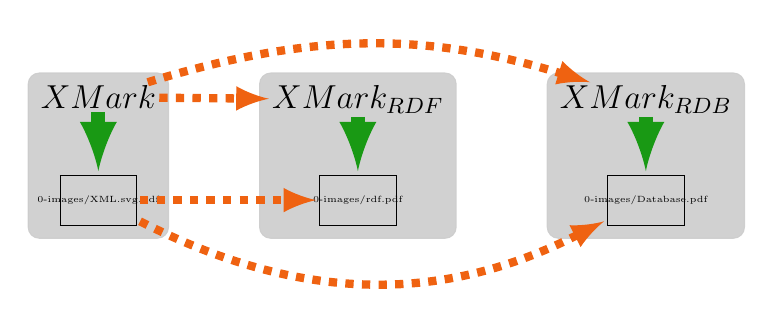
\begin{tikzpicture}
    \matrix<+->[ampersand replacement=\&, column sep = 4em, matrix of nodes,row sep=2em,inner sep=.1em] (xmark){
      $XMark$ \&       |[visible on=<+->]|$XMark_{RDF}$ \&  |[visible on=<+->]|     $XMark_{RDB}$ \\
      \scalebox{.65}{\pgfuseimage{xml}} \& |[visible on=<.(-1)->]|\scalebox{.65}{\pgfuseimage{rdf}} \& |[visible on=<.->]|\scalebox{.65}{\pgfuseimage{rdb}} \\
    };

    \begin{pgfonlayer}{background}
      \node[box=gray,visible on=<.(-2)->,fit={(xmark-1-1) (xmark-2-1)}] {} ;%
      \node[box=gray,visible on=<.(-1)->,fit={(xmark-1-2) (xmark-2-2)}] {} ;%
      \node[box=gray,visible on=<.->,fit={(xmark-1-3) (xmark-2-3)}] {} ;%
    \end{pgfonlayer}

    \path[visible on=<.(-2)->,-latex] (xmark-1-1) edge [color=green,line width=5pt] (xmark-2-1); 
    \path[visible on=<.(-1)->,-latex] (xmark-1-2) edge [color=green,line width=5pt] (xmark-2-2); 
    \path[visible on=<.->,-latex] (xmark-1-3) edge [color=green,line width=5pt] (xmark-2-3); 

    \path[visible on=<.(-1)-.>,-latex,dashed] (xmark-1-1) edge [color=orange,line width=3pt] (xmark-1-2); 
    \path[visible on=<.(-1)-.>,-latex,dashed] (xmark-2-1) edge [color=orange,line width=3pt] (xmark-2-2); 

    \path[visible on=<.>,-latex,dashed] (xmark-1-1) edge [color=orange,line width=3pt,bend left=17] (xmark-1-3); 
    \path[visible on=<.>,-latex,dashed] (xmark-2-1) edge [color=orange,line width=3pt,bend right=27] (xmark-2-3); 

    \end{tikzpicture}
  \end{center}

  \vspace{-10pt}

  \begin{block}<+->{Experimental Results}
    \begin{itemize}
    \item Compared to native XQuery (XMark)
      \begin{description}
      \item[RDB and RDF:] same order of magnitude for most queries
      \end{description}
    \item<+-> Except on RDF nested queries (self joining data)
      \begin{itemize}
      \item[] several orders of magnitude slower
      \item[] due to the number of calls to the SPARQL engine
      \end{itemize}
    \end{itemize}
  \end{block}

\end{frame}


\begin{frame}{Rewriting techniques for Nested Queries}

  \begin{block}<+->{{\small $Q_8$: ``List the names of persons and the number of items they bought.''}}
    \begin{tikzpicture}
      \node[text width=\linewidth] {
        \VerbatimInput{queries/query08.xsparql}
      };

      \begin{pgfonlayer}{background}
        \draw[box,visible on=<+-.(6)>] (-0.51\linewidth,4em) rectangle (0em,2em);
      \end{pgfonlayer}

      \node[boxFull=green,visible on=<.-.(3)>,text width=3.8cm,anchor=west] at (2em,5em) 
      {Returns $\left(\begin{array}{c} {\texttt{\scriptsize nuno}},\\ {\texttt{\scriptsize axel}},\\ \vdots\end{array} \right)$};
          

      \begin{pgfonlayer}{background}
        \draw[box,visible on=<+->] (-13em,.5em) rectangle (0em,-1.2em);
      \end{pgfonlayer}

      \node[boxFull=green,visible on=<.-.(2)>,text width=5cm,inner sep=0] at (0.25\linewidth,-1em) (rewrite) {\VerbatimInput{queries/nested-inner-rewriting.xq}};

      \node[boxFull=orange,visible on=<+>,text width=1cm,anchor=south west] at (10em,-2.4em) {{\scriptsize\tt nuno}};
      \node[boxFull=orange,visible on=<.>,text width=1cm,anchor=south west] at (7em,6em) {{\scriptsize\tt nuno}};

      \begin{scope}[visible on=<+>]
        \node[boxFull=orange,text width=1cm,anchor=south west] at (10em,-2.5em) {{\scriptsize\tt axel}};
        \node[boxFull=orange,text width=1cm,anchor=south west] at (7em,4.5em) {{\scriptsize\tt axel}};
      \end{scope}
    
          

      \path[visible on=<+>,-latex,dashed] (0em,0em) edge [color=orange,line width=3pt,bend right] (0em,4.5em); 

      \node[boxFull=green,visible on=<.-.(1)>,text width=5.5cm,anchor=south east] at (0em,4.5em) {\VerbatimInput{queries/nested-inner-rewriting-opt.xq}};
      \draw[draw=none,fill=beamer@lightblendedgreen,visible on=<+->] (-13.1em,.6em) rectangle (.1em,-1.3em) node[midway] {Join in XQuery};

      \node[boxFull=green,visible on=<+>,text width=4cm,anchor=north west] at (.1em,4em) {Nested Loop rewriting};
      \node[visible on=<.->,text width=5.5cm,anchor=south east] at (0em,4.5em) {\VerbatimInput{queries/nested-inner-rewriting-opt.xq}};

      % other optimisations
      \node[boxFull=green,visible on=<+>,text width=5cm,anchor=north west] at (.1em,0em) {Applied to related language: SPARQL2XQuery~\cite{GroppeGroppeLinnemann:2008aa}};

      \node[boxFull=green,visible on=<+>,text width=5cm,anchor=north west] at (.1em,0em) {Other optimisations: \\ Join in SPARQL};
      

    \end{tikzpicture}
  \end{block}

\end{frame}


\def\plotsDir{1-xsparql/plots/}
%
\begin{frame}{Evaluation of different rewritings - $XMark_{RDF} Q_8$}
  \pgfplotsset{
    tick label style={font=\small},
    label style={font=\small},
    legend style={font=\footnotesize}
  }
  \begin{figure}
    \setlength{\abovecaptionskip}{0pt}
    \setlength{\belowcaptionskip}{0pt}
      \import{\plotsDir}{optimisations-paper-query08}
    \vspace{-5pt}
  \end{figure}

  \vspace{-5pt}
  \begin{block}{}
    \begin{itemize}
    \item Optimised rewritings show promising results
    \item Best Results: SPARQL-based 
    \item Results included in~\cite{BischofDeckerKrennwallner:2012aa}
    \end{itemize}
  \end{block}
\end{frame}


\begin{frame}{Evaluation of different rewritings - $XMark_{RDB} Q_8$}
  \pgfplotsset{
    tick label style={font=\small},
    label style={font=\small},
    legend style={font=\footnotesize}
  }
  {
    \begin{figure}
      \setlength{\abovecaptionskip}{0pt}
      \setlength{\belowcaptionskip}{0pt}
      \import{\plotsDir}{optimisations-paper-query08-rdb}
      \vspace{-5pt}
    \end{figure}
  }
  \vspace{-5pt}
  \begin{block}{}
    \begin{itemize}
    \item Not so effective for RDB, requires different optimisations
    \item Due to schema representation?
    \item Additional Results for this thesis
    \end{itemize}
  \end{block}
\end{frame}



%%% Local Variables:
%%% mode: latex
%%% mode: flyspell
%%% mode: reftex
%%% TeX-master: "../presentation"
%%% End:


\section{Annotated RDF(S)}
\subsection*{Overview}



\begin{frame}{Data Integration: Pizza Delivery Company} 

  \hspace*{-1em}
  \begin{tikzpicture}

    \begin{scope}[visible on=<+->]
      \node (rdb) at (5,-2) {\pgfuseimage{rdb}} ;
      \node at (rdb.north east) {\pgfuseimage{rdb-table}}; 
      \node[box=green,visible on=<.->] at (rdb.north west) {RDB};
      \node[inner sep=0,left=.1em of rdb.west] (rdb-name1) {Clients};
      \node[inner sep=0,below=.1em of rdb-name1.south] (rdb-name) {/ Orders};
      
      \begin{pgfonlayer}{background}
        \node[box=gray, fit=(rdb) (rdb-name)] (rdbms) {} ;
      \end{pgfonlayer}

    \end{scope}


    \begin{scope}
      \node at (-4,-2) (excel) {\pgfuseimage{excel}};

      \node[inner sep=0] at (excel.south) (excel-name) {Deliveries};
      
      \begin{pgfonlayer}{background}
        \node[box=gray, visible on =<.->, fit=(excel) (excel-name)] {} ;
      \end{pgfonlayer}

      \node at (excel.north east) {\scalebox{.7}{\pgfuseimage{xml}}};
      \node[box=green,visible on=<.->] at (excel.north west) {XML};

    \end{scope}
    
    \begin{scope}
      \node (eat) at (-4,3){\pgfuseimage{eat}};
      \node[inner sep=0,below=.1em of eat.south] (eat-name1) {Clients};
      \node[inner sep=0,below=.1em of eat-name1.south] (eat-name) {/ Orders};

      \begin{pgfonlayer}{background}
        \node[box=gray, visible on =<.->, fit=(eat) (eat-name)] {} ;
      \end{pgfonlayer}

      \node at (eat.north east) {\scalebox{.7}{\pgfuseimage{xml}}};
      \node[box=green,visible on=<.->] at (eat.north west) {XML};

    \end{scope}


    \begin{scope}
      \node at (1,1) (di)  {\pgfuseimage{XSPARQLogo}};
      
      \path[-latex] (eat.south east) edge [color=xquery,line width=5pt] (di); 
      \path[-latex] (rdb.north west) edge [color=xquery,line width=5pt] (di); 
      \path[-latex] (excel.north east) edge [color=xquery,line width=5pt] (di); 
      
    \end{scope}
    
    \begin{scope}
      \node at (5,3) (dbpedia)  {\pgfuseimage{dbpedia}};

      \begin{pgfonlayer}{background}
        \node[box=gray, visible on =<.->, fit=(dbpedia)] {} ;
      \end{pgfonlayer}

      \node at (dbpedia.north east) {\scalebox{.7}{\pgfuseimage{rdf}}};
      \node[box=green,visible on=<.->] at (dbpedia.north west) {RDF};

      \path[latex-latex] (dbpedia.south west) edge [color=xquery,line width=5pt] (di);

    \end{scope}



    \begin{scope}[visible on=<+->]
      \node[boxFull=green,text width=3cm] at (rdb.south west) (rdb-order){
        {\small
          \begin{tabular}{c|c}
            person & address\\
            \hline
            Nuno & Galway \\
          \end{tabular}
        }
      };
      
      \node[boxFull=green,text width=4.2cm,anchor=north] at (eat.south east) (eat-order){
        \VerbatimInput[firstline=2,lastline=5]{queries/justeat.xml}
      };

    \end{scope}

    \begin{scope}[visible on=<.->]
      \node[boxFull=red,anchor=north] at (eat-order.south){2012};
      \node[boxFull=red,anchor=south] at (rdb-order.north){From 2008 to 2012};
    \end{scope}
    
  \end{tikzpicture}

\end{frame}



 
\begin{frame}{Use Annotated RDF(S)!}

  \begin{center}
    Annotations refer to a specific \alert{\textbf{domain}}
  \end{center}
  \pause
  {\color{green}{Temporal:}}\\[-.6em]
  \begin{block}{}
    {\small\tt
      :nuno :address :Galway . \textcolor{blue}{[2008,2012]}
    }
  \end{block}
  \pause

  {\color{green}{Fuzzy:}}\\[-.6em]
  \begin{block}{}
    {\small\tt
      :nuno :address :Dublin . \textcolor{blue}{0.9}
    }
  \end{block}

  \pause

  {\color{green}{Provenance:}}\\[-.5em]
  \begin{block}{}
    {\small\tt
      :nuno :address :Dublin . \textcolor{blue}{<http://eat.ie>}
    }
  \end{block}

  \pause
  \begin{center}
    Representation for the \textcolor{blue}{values} of each \alert{annotation domain}
  \end{center}

  
\end{frame}



\subsection{Annotated RDFS}



\begin{frame}[fragile]{Annotated RDF(S) Inference example}
     \vspace{-10pt}
     \begin{center}
       Inference rules are \alert{\textbf{independent}} of the annotation domain
     \end{center}
     \vspace{-10pt}
    \uncover<2->{
      \begin{block}{\only<3->{\alert<3>{Annotated}} RDFS subPropertyOf (``\texttt{\spp}'') rule:}
      {\small\tt\begin{tabbing}
          \(\Rightarrow\) \=:x ?Prop2 ?y \= \only<3->{\alert<3>{?\(v{1} \otimes v{2}\)}}\kill
          \> ?Prop1 \spp\ ?Prop2 .\ \ \=\only<3->{\alert<3>{?\(v{1}\)}}\\
          \> ?x ?Prop1 ?y .\> \only<3->{\alert<3>{?\(v{2}\)}}  \\
          \(\Rightarrow\) \> ?x ?Prop2\ ?y .\> \only<4->{?v{1}\ \alert<4>{\(\otimes\)}\ ?v{2}}
        \end{tabbing}}
    \end{block}

       \begin{block}{}
         {\small\tt
        \begin{tabbing}
          \(\Rightarrow\) \=:address foaf:based\_Near\ :room311\=\kill
          \>:address \spp\ foaf:based\_near .\> \only<3->{\alert<3>{[2009,\(+\infty\)]}}\\          
          \>:nuno :address :Galway  .\> \only<3->{\alert<3>{[2008,2012]}}\\
          \(\Rightarrow\) \>:nuno foaf:based\_near\ :Galway .\> \only<4->{{[2009,\(+\infty\)]{\alert<4>{\(\otimes\)}}[2008,2012]}}
        \end{tabbing}}
    \end{block}
  }

  \begin{block}<5->{ Extra rule to group annotations triples ($\oplus$):}
    {\small\tt
      \begin{tabbing}
      \(\Rightarrow\) \=:nuno :address :Galway \ \ \ \ \  \=\kill
      \> \uncover<5-6>{:nuno :address :Galway .}\> \uncover<5-6>{[2009,\(+\infty\)]}\\
      \> \uncover<5-6>{:nuno :address :Galway .}\> \uncover<5-6>{[2008,2012]}\\
      \only<6,7->{\(\Rightarrow\) \> :nuno :address :Galway .\>  [2009,\(+\infty\)]\alert<6>{\(\oplus\)}[2008,2012]}
    \end{tabbing}}
\end{block}

\end{frame}


%%% Local Variables:
%%% mode: latex
%%% mode: flyspell
%%% mode: reftex
%%% TeX-master: "../presentation"
%%% End:



\begin{frame}{Operations on Annotations Elements}

  \begin{block}{}
    \begin{center}
      \begin{tikzpicture}
        \matrix[ampersand replacement=\&,matrix of nodes,row sep=2em,column sep=0em] (lat) {
          \&|[visible on=<5>]| $[-\infty,+\infty]$ \& \\
          \&|[visible on=<4->, text width=2cm]| $\only<-7>{\visible<-5>{[2008,+\infty]}}\only<8->{\hspace{-30pt}\visible<9>{\alert{\{}}[2000,2005],[2008,2012]\visible<9>{\alert{\}}}}$ \& \\ 
          $\visible<9>{\alert{\{}}[\only<-5>{2009,+\infty}\only<6->{\alert<6>{2000,2005}}]\visible<9>{\alert{\}}}$ \& \& $\visible<9>{\alert{\{}}[2008,2012]\visible<9>{\alert{\}}}$\\
          \&|[visible on=<2-5>]| $\visible<9>{\alert{\{}}[2009,2012]\visible<9>{\alert{\}}}$ \& \\
          \&|[visible on=<3->]| $\invisible<6>{\visible<9>{\alert{\{}}[]\visible<9>{\alert{\}}}}$ \& \\
        };

        \begin{scope}[visible on=<2-5>]
          \path (lat-4-2) edge (lat-3-1);
          \path (lat-4-2) edge (lat-3-3);
          \node[above=.5em of lat-4-2] {\alert<2>{$\otimes$}};
        \end{scope}
        \path[visible on=<3-5>] (lat-4-2) edge[dashed] (lat-5-2);

        \begin{scope}[visible on=<7->]
          \path (lat-5-2) edge (lat-3-1);
          \path (lat-5-2) edge (lat-3-3);
          \node[above=.5em of lat-5-2] {\alert<2>{$\otimes$}};
        \end{scope}
        
        \begin{scope}[visible on=<4-5>]
          \path (lat-2-2) edge (lat-3-1);
          \path (lat-2-2) edge (lat-3-3);
          \node[below =.5em of lat-2-2] {\alert<3>{$\oplus$}};
        \end{scope}
        \path[visible on=<5>] (lat-1-2) edge[dashed] (lat-2-2);

        \begin{scope}[visible on=<8->]
          \path (lat-2-2) edge (lat-3-1);
          \path (lat-2-2) edge (lat-3-3);
          \node[below =.5em of lat-2-2] {$\oplus$};
        \end{scope}

      \end{tikzpicture}
    \end{center}
  \end{block}

\end{frame}




\subsection{AnQL: Annotated SPARQL}

\begin{frame}[fragile]{AnQL: Annotated SPARQL}

  \begin{block}{Extension of SPARQL Syntax}
    \begin{itemize}
    \item<+-> \alert<.>{triple pattern}
    \item<+-> \alert{annotated triple pattern} is a triple pattern plus 
      \begin{itemize}
      \item<.-> annotation term\only<+->{; or}
      \item<.-> annotation variable
      \end{itemize}
    \item<+-> \alert{Basic Annotated Patterns} (BAP) are sets of annotated triple patterns

    \end{itemize}
  \end{block}

  \begin{block}{Example}
    \begin{small}
      \begin{semiverbatim}
\only<4->{\{} \uncover<-2,4->{?person a foaf:Person . \only<2,4->{[\(-\infty, +\infty\)]}}\only<-2>{
}
  \only<3->{?person :address ?address . ?l 
\uncover<4->{\}}} 
\end{semiverbatim}
    \end{small}
  \end{block}

\visible<+->{Combine BAPs using $\mathsf{AND} (.)$, $\mathsf{OPTIONAL}$, $\mathsf{UNION}$, $\mathsf{FILTER}$}

 
\end{frame}



%%% Local Variables:
%%% mode: latex
%%% mode: flyspell
%%% mode: reftex
%%% TeX-master: "../presentation"
%%% End:





\begin{frame}[fragile]{Evaluation of SPARQL OPTIONALs}

  \begin{block}{\small ``List my  address, time interval and optionally people living in the same city at the same time.''}
    \begin{Verbatim}[frame=none,fontsize=\small]
SELECT   ?city ?t ?person 
WHERE    { :nuno :address ?city . ?t
           OPTIONAL { ?person :address ?city . ?t } }
    \end{Verbatim}
  \end{block}

  \begin{block}{Sample input:}
    {\small\tt
    $\begin{array}{llll}
      \term{{:}nuno} & \term{{:}address} & \term{{:}Galway}\ . & \alert<2,3>{\ [2008, 2012]}\\
      {\color<3>{blue}{\term{{:}axel}}} & \term{{:}address} & \term{{:}Galway}\ . & \alert<3>{\ [2005, 2010]}\\
    \end{array}$
  }
  \end{block}
  \pause 

  \begin{block}{Answers:}
    $\begin{array}{lcl}
      S_{1} & = & \{?city \to \term{{:}Galway}, ?t \to \alert<2>{[2008, 2012]}\} \\ 
      \pause 
      S_{2} & = & \{?city \to \term{{:}Galway}, ?t \to \alert<3>{[2008, 2010]}, \  ?person \to {\color<3>{blue}{\term{{:}axel}}}\} \\ 
    \end{array}$
  \end{block}
  
  \pause

  {\small \alert{OPTIONAL provide more information maybe restricting annotation values}}

\end{frame}


\begin{frame}{Annotated RDF(S) Domains}

  {\color{green}{Temporal:}}\\[-.6em]
  \begin{block}{}
    {\small\tt
      :nuno :address :Galway . \textcolor{blue}{[2008,2012]}
    }
  \end{block}

  {\color{green}{Fuzzy:}}\\[-.6em]
  \begin{block}{}
    {\small\tt
      :nuno :address :Galway . \textcolor{blue}{0.9}
    }
  \end{block}

  {\color{green}{Provenance:}}\\[-.5em]
  \begin{block}{}
    {\small\tt
      :nuno :address :Dublin . \textcolor{blue}{http://eat.ie}
    }
  \end{block}


  \pause
  {\color{green}{Combining domains:}} Included in~\cite{ZimmermannLopesPolleres:2012aa}\\[-.5em]
  \begin{block}{}
    {\small\tt
      :nuno :address :Dublin . \textcolor{blue}{(http://eat.ie, [2012,2012])}
    }
  \end{block}

  \pause
  {\color{green}{Access Control:}} Presented at~\cite{LopesKirraneZimmermann:2012aa}\\[-.5em]
  \begin{block}{}
    {\small\tt
      :nuno :address :Galway . \textcolor{blue}{[nl]}
    }
  \end{block}

  
\end{frame}




%%% Local Variables:
%%% mode: latex
%%% mode: flyspell
%%% mode: reftex
%%% TeX-master: "../presentation"
%%% End:




\subsection{Architecture}


\begin{frame}{Architecture combining XSPARQL and AnQL}

  \begin{center}
    
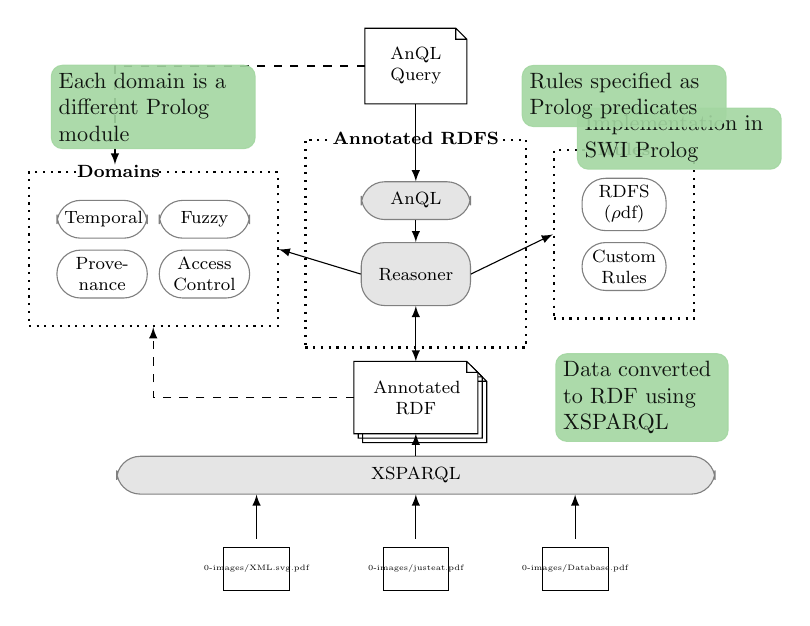
\begin{tikzpicture}[node distance = 35pt,scale=.8,transform shape,%
  terminal/.style={ rectangle,minimum size=6mm,rounded corners=3mm,text centered,draw=black!50,fill=gray!20},%
  component/.style={ rectangle,minimum size=6mm,rounded corners=3mm,text centered,draw=black!50},%
  rdb/.style={cylinder, shape border rotate=90, draw,minimum width=1.5cm,minimum height=1cm, shape aspect=.35}%
  ]

  \tikzstyle{every node}=[font=\footnotesize]

  % reasoner
  \begin{scope}[visible on=<2->]
    \node[terminal, text width=1.5cm, minimum height=1cm] (reasoner) {Reasoner}; %
    \coordinate[left= 5em of reasoner.west] (left-reasoner);
  \end{scope}
  
  % domains
  \begin{scope}[node distance = 5pt,text width=1.2cm,anchor=east,visible on=<3->]

    \node[component] at (left-reasoner) (ac) {Access Control}; %
    \node[component, above=of ac]  (frdf) {Fuzzy}; %
    \node[component,left =of frdf] (trdf) {Temporal}; %
    \node[component,below =of trdf] (prov) {Prove\-nance}; %

    % domains outer box
    \node[draw=black,dotted,thick,inner sep=10pt,rectangle,fit=(trdf) (ac) (frdf) (prov)] (domains) {} ;%
    \node[,inner sep=0,fill=white] at (domains.north) (domains-label) { \bf Domains};
  \end{scope}



  \coordinate[right= 5em of reasoner.north east] (right-reasoner);
  % rules outer box
  \begin{scope}[visible on=<4->]
    % domains
    \begin{scope}[node distance = 5pt,text width=1.1cm,anchor=north west]
      \node[component] at (right-reasoner) (crules) {Custom Rules}; %
      \node[component, above=of crules]  (rhodf) {RDFS ($\rhodf$)}; %
    \end{scope}
    
    \node[draw=black,dotted,thick,inner sep=10pt,rectangle,fit=(rhodf) (crules)] (rules) {} ;%
    \node[inner sep=0,fill=white] at (rules.north) {\bf Rules};
    \draw[-latex] (reasoner.east) -- (rules.west);%

  \end{scope}


  % anql 
  \begin{scope}[visible on=<2->]
    \node[terminal,text width=1.5cm, above =1em of reasoner] (anql) {AnQL}; %
    \node[draw=black,dotted,thick,inner ysep=15pt,inner xsep=20pt,rectangle,fit=(anql) (reasoner)] (ardf) {} ;%
    
    \node[inner sep=0,fill=white] at (ardf.north) (ardfs) { \bf Annotated RDFS};
    \draw[latex-] (reasoner.north) -- (anql.south);%
  \end{scope}
  
  \begin{scope}[visible on=<5->]
    \node[doc, above = of anql] (anqlQuery) {AnQL Query}; %
    \draw[-latex] (anqlQuery.south) -- (anql.north);%
    \draw[dashed,-latex] (anqlQuery.west) -| (domains-label.north);%
  \end{scope}




  % input sources
  \documentSetL{below=2.5em of reasoner}{ardf}{Annotated RDF};%

  \begin{scope}[visible on=<3->]
    \draw[dashed,-latex] (ardf.west) -| (domains.south);%
    \draw[-latex] (reasoner.west) -- (domains.east);%
  \end{scope}
  
  \draw[visible on=<2->,latex-latex] (reasoner.south) -- (ardf.north);%

 

  \node[terminal,below =1em  of ardf,minimum width=9.5cm] (xsparql) {XSPARQL}; %
  \draw[-latex] ($(xsparql.north west)!(ardf.south)!(xsparql.north east)$) -- (ardf.south);%

 
  \node[below=2em of xsparql]  (crm)  {\scalebox{.7}{\pgfuseimage{eat}}};%
  \draw[-latex] (crm.north) -- (xsparql.south);%


  \node[left=of crm]  (hr)  {\scalebox{.7}{\pgfuseimage{xml}}};%
  \draw[-latex] (hr.north) -- ($(xsparql.south west)!(hr.north)!(xsparql.south east)$);%


  \node[right=of crm]  (dms)  {\scalebox{.7}{\pgfuseimage{rdb}}};%
  \draw[-latex] (dms.north) -- ($(xsparql.south west)!(dms.north)!(xsparql.south east)$);%

  

    \node[box=green,visible on=<1>,text width=2.5cm, font=\normalsize, right =of ardf]  {Data converted to RDF using XSPARQL};


    \node[box=green,visible on=<2>,text width=3cm, font=\normalsize,right =of ardfs]  {Implementation in SWI Prolog};


    \node[box=green,visible on=<3>,text width=3cm, font=\normalsize,anchor=south,above=1em of domains]  {Each domain is a different Prolog module};


    \node[box=green,visible on=<4>,text width=3cm, font=\normalsize,anchor=south,above =1em of rules] {Rules specified as Prolog predicates};



\end{tikzpicture}



%%% Local Variables:
%%% mode: latex
%%% mode: flyspell
%%% mode: reftex
%%% TeX-master: "../presentation"
%%% End:


  \end{center}

\end{frame}



%%% Local Variables:
%%% mode: latex
%%% mode: flyspell
%%% mode: reftex
%%% TeX-master: "../presentation"
%%% End:




%%% Local Variables:
%%% mode: latex
%%% mode: flyspell
%%% mode: reftex
%%% TeX-master: "../presentation"
%%% End:




\section{Conclusions}

\subsection{}


\begin{frame}{Conclusions}


  \begin{block}{}
    Efficient data integration over heterogenous data sources can be achieved by
    \begin{enumerate}
    \item<2-> a combined query language that accesses heterogenous data in its original sources
      \begin{itemize}
      \item<3-| alert@3> XSPARQL can integrate heterogeneous sources
      \end{itemize}
    \item<2-> optimisations for efficient query evaluation for this language
      \begin{itemize}
      \item<4-| alert@4> rewriting techniques for nested queries for our implementation of XSPARQL
      \end{itemize}
    \item<2-> an RDF-based format with support for context information
      \begin{itemize}
      \item<5-| alert@5> Annotated RDFS: inferences and query over context information 
      \item<5-| alert@5> Use XSPARQL to create Annotated RDF representing the integrated data
      \end{itemize}
    \end{enumerate}
  \end{block}
  
  \visible<6->{
    \begin{center}
      \begin{Large}
        \alert{Thank you! Questions?}
      \end{Large}
    \end{center}
  }

\end{frame}

%%% Local Variables:
%%% mode: latex
%%% mode: flyspell
%%% mode: reftex
%%% TeX-master: "presentation"
%%% End:


\newcounter{finalframe}
\setcounter{finalframe}{\value{framenumber}}

\appendix

\section*{Bibliography}
{
  \setbeamertemplate{footline}{}
  \addtocounter{framenumber}{-1}
  \begin{frame}[allowframebreaks]{Bibliography}
    \def\newblock{}
\begin{thebibliography}{BDK{\etalchar{+}}12}

% \bibitem[JoDS2012]{BischofDeckerKrennwallner:2012aa}
\bibitem[JoDS2012]{BischofDeckerKrennwallner:2012aa}
Stefan Bischof, Stefan Decker, Thomas Krennwallner, Nuno Lopes, and Axel
  Polleres.
\newblock {Mapping between RDF and XML with XSPARQL}.
\newblock {\em Journal on Data Semantics}, 1:147--185, 2012.

% \bibitem[GGL{\etalchar{+}}08]{GroppeGroppeLinnemann:2008aa}
\bibitem[SAC2008]{GroppeGroppeLinnemann:2008aa}
Sven Groppe, Jinghua Groppe, Volker Linnemann, Dirk Kukulenz, Nils Hoeller, and
  Christoph Reinke.
\newblock {Embedding SPARQL into XQuery/XSLT}.
\newblock In Roger~L. Wainwright and Hisham Haddad, editors, {\em {Proceedings
  of the 2008 ACM Symposium on Applied Computing (SAC), Fortaleza, Ceara,
  Brazil, March 16-20, 2008}}, pages 2271--2278. ACM, 2008.

% \bibitem[LBDP11]{LopesBischofDecker2011aa}
\bibitem[EPIA2011]{LopesBischofDecker2011aa}
Nuno Lopes, Stefan Bischof, Stefan Decker, and Axel Polleres.
\newblock {On the Semantics of Heterogeneous Querying of Relational, XML and
  RDF Data with XSPARQL}.
\newblock In Paulo Moura and Vitor~Beires Nogueira, editors, {\em {Proceedings
  of the 15th Portuguese Conference on Artificial Intelligence (EPIA2011) --
  Computational Logic with Applications Track}}, Lisbon, Portugal, October
  2011.

% \bibitem[LKZ{\etalchar{+}}12]{LopesKirraneZimmermann:2012aa}
\bibitem[ICLP2012]{LopesKirraneZimmermann:2012aa}
Nuno Lopes, Sabrina Kirrane, Antoine Zimmermann, Axel Polleres, and Alessandra
  Mileo.
\newblock {A Logic Programming approach for Access Control over RDF}.
\newblock In Agostino Dovier and V{\'\i}tor~Santos Costa, editors, {\em
  {Technical Communications of the 28th International Conference on Logic
  Programming (ICLP'12)}}, volume~17 of {\em Leibniz International Proceedings
  in Informatics (LIPIcs)}, pages 381--392, Dagstuhl, Germany, 2012. Schloss
  Dagstuhl--Leibniz-Zentrum fuer Informatik.

\bibitem[ISWC2010]{LopesPolleresStraccia:2010aa}
Nuno Lopes, Axel Polleres, Umberto Straccia, and Antoine Zimmermann.
\newblock {AnQL: SPARQLing Up Annotated RDFS}.
\newblock In {\em {International Semantic Web Conference (1)}}, pages 518--533,
  2010.

\bibitem[AAAI2010]{StracciaLopesLukacsy:2010aa}
Umberto Straccia, Nuno Lopes, Gergely Luk{\'a}csy, and Axel Polleres.
\newblock {A General Framework for Representing and Reasoning with Annotated
  Semantic Web Data}.
\newblock In Maria Fox and David Poole, editors, {\em {Proceedings of the
  Twenty-Fourth AAAI Conference on Artificial Intelligence, AAAI 2010, Atlanta,
  Georgia, USA, July 11-15, 2010}}. AAAI Press, July 2010.

\bibitem[JWS2012]{ZimmermannLopesPolleres:2012aa}
Antoine Zimmermann, Nuno Lopes, Axel Polleres, and Umberto Straccia.
\newblock {A General Framework for Representing, Reasoning and Querying with
  Annotated Semantic Web Data}.
\newblock {\em Web Semantics: Science, Services and Agents on the World Wide
  Web}, 11(0):72--95, 2012.

\end{thebibliography}

  \end{frame}
}


\setcounter{framenumber}{\value{finalframe}}

\end{document}

%%% Local Variables:
%%% mode: latex
%%% mode: flyspell
%%% mode: reftex
%%% End:
